\documentclass[12pt]{article}
\usepackage[spanish]{babel}
\usepackage[utf8]{inputenc}
\usepackage[T1]{fontenc}
\usepackage{geometry}
\usepackage{setspace}
\usepackage{graphicx}
\usepackage[colorlinks=true, linkcolor=blue, citecolor=blue, urlcolor=blue]{hyperref}
\usepackage{listings}
\usepackage{xcolor}
\usepackage{float}
\usepackage{booktabs}
\usepackage{enumitem}
\definecolor{codebg}{RGB}{245,245,245}
\definecolor{codekeyword}{RGB}{0,0,180}
\definecolor{codecomment}{RGB}{95,140,95}
\definecolor{codestring}{RGB}{163,21,21}
\lstdefinestyle{bashStyle}{
    backgroundcolor=\color{codebg},
    commentstyle=\color{codecomment}\itshape,
    keywordstyle=\color{codekeyword}\bfseries,
    stringstyle=\color{codestring},
    basicstyle=\ttfamily\small,
    breakatwhitespace=false,
    breaklines=true,
    captionpos=b,
    keepspaces=true,
    numbers=none,
    showspaces=false,
    showstringspaces=false,
    showtabs=false,
    tabsize=2,
    frame=single,
    rulecolor=\color{gray!40},
    language=bash
}
\lstdefinestyle{sqlStyle}{
    backgroundcolor=\color{codebg},
    commentstyle=\color{codecomment}\itshape,
    keywordstyle=\color{codekeyword}\bfseries,
    stringstyle=\color{codestring},
    basicstyle=\ttfamily\small,
    breakatwhitespace=false,
    breaklines=true,
    captionpos=b,
    keepspaces=true,
    numbers=none,
    showspaces=false,
    showstringspaces=false,
    showtabs=false,
    tabsize=2,
    frame=single,
    rulecolor=\color{gray!40},
    language=SQL,
    morekeywords={SERIAL}
}
\lstset{style=sqlStyle}
\lstdefinestyle{panel}{
  backgroundcolor=\color{gray!8},
  basicstyle=\ttfamily\footnotesize,
  frame=single,
  framerule=0.4pt,
  rulecolor=\color{gray!50},
  numbers=none,
  breaklines=true,
  columns=fullflexible,
  showstringspaces=false,
  xleftmargin=12pt,
  xrightmargin=12pt,
  aboveskip=10pt,
  belowskip=10pt
}
\geometry{letterpaper, margin=1in}
\setstretch{1.25}
\usepackage[
  backend=biber,
  style=ieee,
  doi=true,
  url=true
]{biblatex}
\DeclareFieldFormat{doi}{\href{https://doi.org/#1}{#1}}
\addbibresource{Referencias.bib}
\setlength{\parindent}{0pt}
\setlength{\parskip}{6pt}
\begin{document}
\pagestyle{empty}
\renewcommand{\tablename}{Tabla}

% ============================================================
%  CARÁTULA
% ============================================================
\begin{titlepage}
\thispagestyle{empty}
\centering
\vspace*{0.3cm}


\includegraphics[width=4.2cm]{logo_uteq.png}

\vspace{1cm}

{\Large \textbf{UNIVERSIDAD TÉCNICA ESTATAL DE QUEVEDO}}\par
{\small TEMA:}\par
\vspace{0.1cm}
{\large \textbf{Tercera Entrega del Proyecto Fin de Curso (PFC) \\ Sistema de Gestión de Recursos Operativos, Administrativos y de Seguridad (SGROAS)}}\par

\vspace{0.3cm}
{\footnotesize GRUPO CET:}\par
\vspace{0.3cm}
{\small \textbf{CASTRO ESPINOZA KEVIN MOISES}}\par
{\small \textbf{ESCUDERO PLAZA MARIA DEL ROSARIO}}\par
{\small \textbf{TEJADA BAJAÑA LUIS ALEJANDRO}}\par

\vspace{0.3cm}
{\small \textbf{DOCENTE:}}\par
\vspace{0.3cm}
{\small \textbf{DR. GLEISTON CICERÓN GUERRERO ULLOA, PH.D.}}\par

\vspace{0.3cm}
{\small \textbf{CURSO:}}\par
\vspace{0.3cm}
{\small \textbf{5TO SOFTWARE A}}\par

\vspace{0.3cm}
{\small \textbf{FECHA:}}\par
\vspace{0.3cm}
{\small \textbf{VIERNES, 24 DE JULIO DEL 2026}}\par

\vfill
\end{titlepage}

\pagestyle{plain}
\setcounter{page}{1}

% ============================================================
%  TABLA DE CONTENIDOS
% ============================================================
\tableofcontents
\clearpage

% ============================================================
%  RESUMEN EJECUTIVO
% ============================================================
\section*{Resumen ejecutivo}
\addcontentsline{toc}{section}{Resumen ejecutivo}

El presente informe documenta el estado del sistema SGROAS (Sistema de Gestión de Recursos
Operativos, Administrativos y de Seguridad) en su hito de Tercera Entrega, correspondiente a la
etiqueta \texttt{v0.9.0-rc} del repositorio \cite{sgroas_repo}. El documento sigue la estructura y
los requisitos técnicos establecidos en la guía institucional de la Tercera Entrega del Proyecto
Fin de Curso (PFC) \cite{uteq2026guia}, consolidando evidencia empírica reproducible sobre el
arranque del sistema, la documentación de la API, el flujo de autenticación JWT, el rendimiento
bajo carga, la cobertura de pruebas y el versionado semántico del repositorio.

% ============================================================
\section{Estado del sistema}

El sistema SGROAS se encuentra operativo en su totalidad mediante orquestación con Docker
Compose. La Figura~\ref{fig:imagen1} evidencia el arranque exitoso de los tres servicios que
componen el sistema (backend, PostgreSQL y Redis) desde un entorno Windows con Docker Desktop.

\begin{figure}[H]
    \centering
    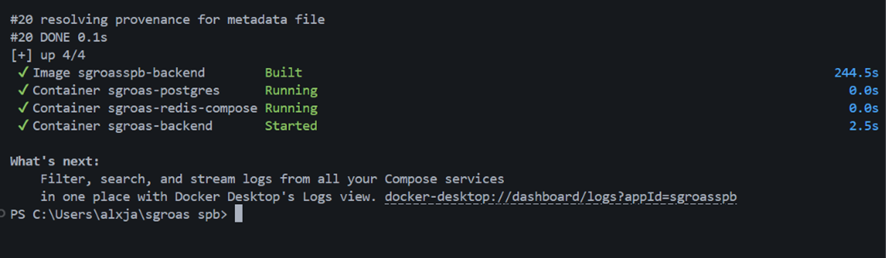
\includegraphics[width=0.85\linewidth]{imagen1}
    \caption{Arranque del sistema completo mediante \texttt{docker compose up}: construcción de
    la imagen del backend y levantamiento de los contenedores \texttt{sgroas-postgres},
    \texttt{sgroas-redis-compose} y \texttt{sgroas-backend}.}
    \label{fig:imagen1}
\end{figure}

El estado de los contenedores en ejecución, con sus puertos publicados y tiempos de actividad,
se confirma en la Figura~\ref{fig:imagen8}, evidenciando que los tres servicios permanecen estables
durante la sesión de pruebas.

\begin{figure}[H]
    \centering
    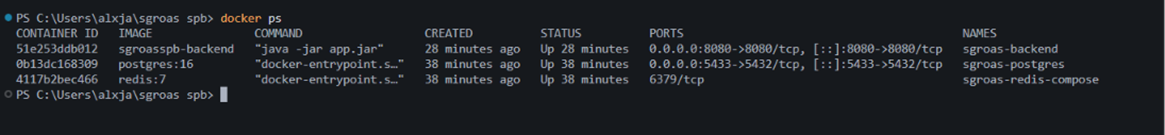
\includegraphics[width=0.85\linewidth]{imagen8}
    \caption{Salida de \texttt{docker ps} confirmando los contenedores
    \texttt{sgroas-backend}, \texttt{sgroas-postgres} y \texttt{sgroas-redis-compose} en
    estado \textit{Up}, con el mapeo de puertos correspondiente.}
    \label{fig:imagen8}
\end{figure}

La documentación interactiva de la API, generada automáticamente mediante Springdoc OpenAPI
3.1 y expuesta en \texttt{/api/docs}, se muestra en la Figura~\ref{fig:imagen2}, cumpliendo el
requisito del Bloque A.1 de la guía de entrega \cite{uteq2026guia}.

\begin{figure}[H]
    \centering
    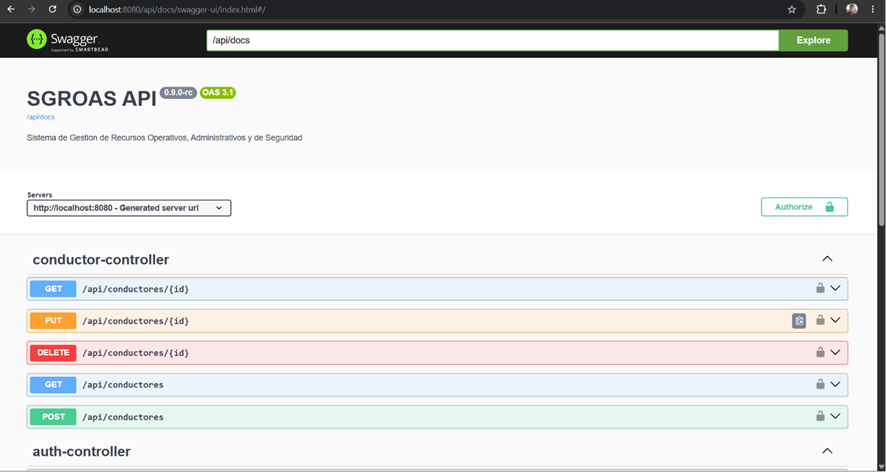
\includegraphics[width=0.85\linewidth]{imagen2}
    \caption{Interfaz Swagger UI de la API SGROAS (versión \texttt{0.9.0-rc}, especificación
    OAS 3.1), mostrando los endpoints del controlador de conductores y del controlador de
    autenticación.}
    \label{fig:imagen2}
\end{figure}

\subsection{Frontend Angular}

La interfaz de usuario del sistema se desarrolló con Angular 20 y se comunica con el backend
mediante cookies HttpOnly para la autenticación. La Figura~\ref{fig:login-frontend} muestra la
pantalla de inicio de sesión.

\begin{figure}[H]
    \centering
    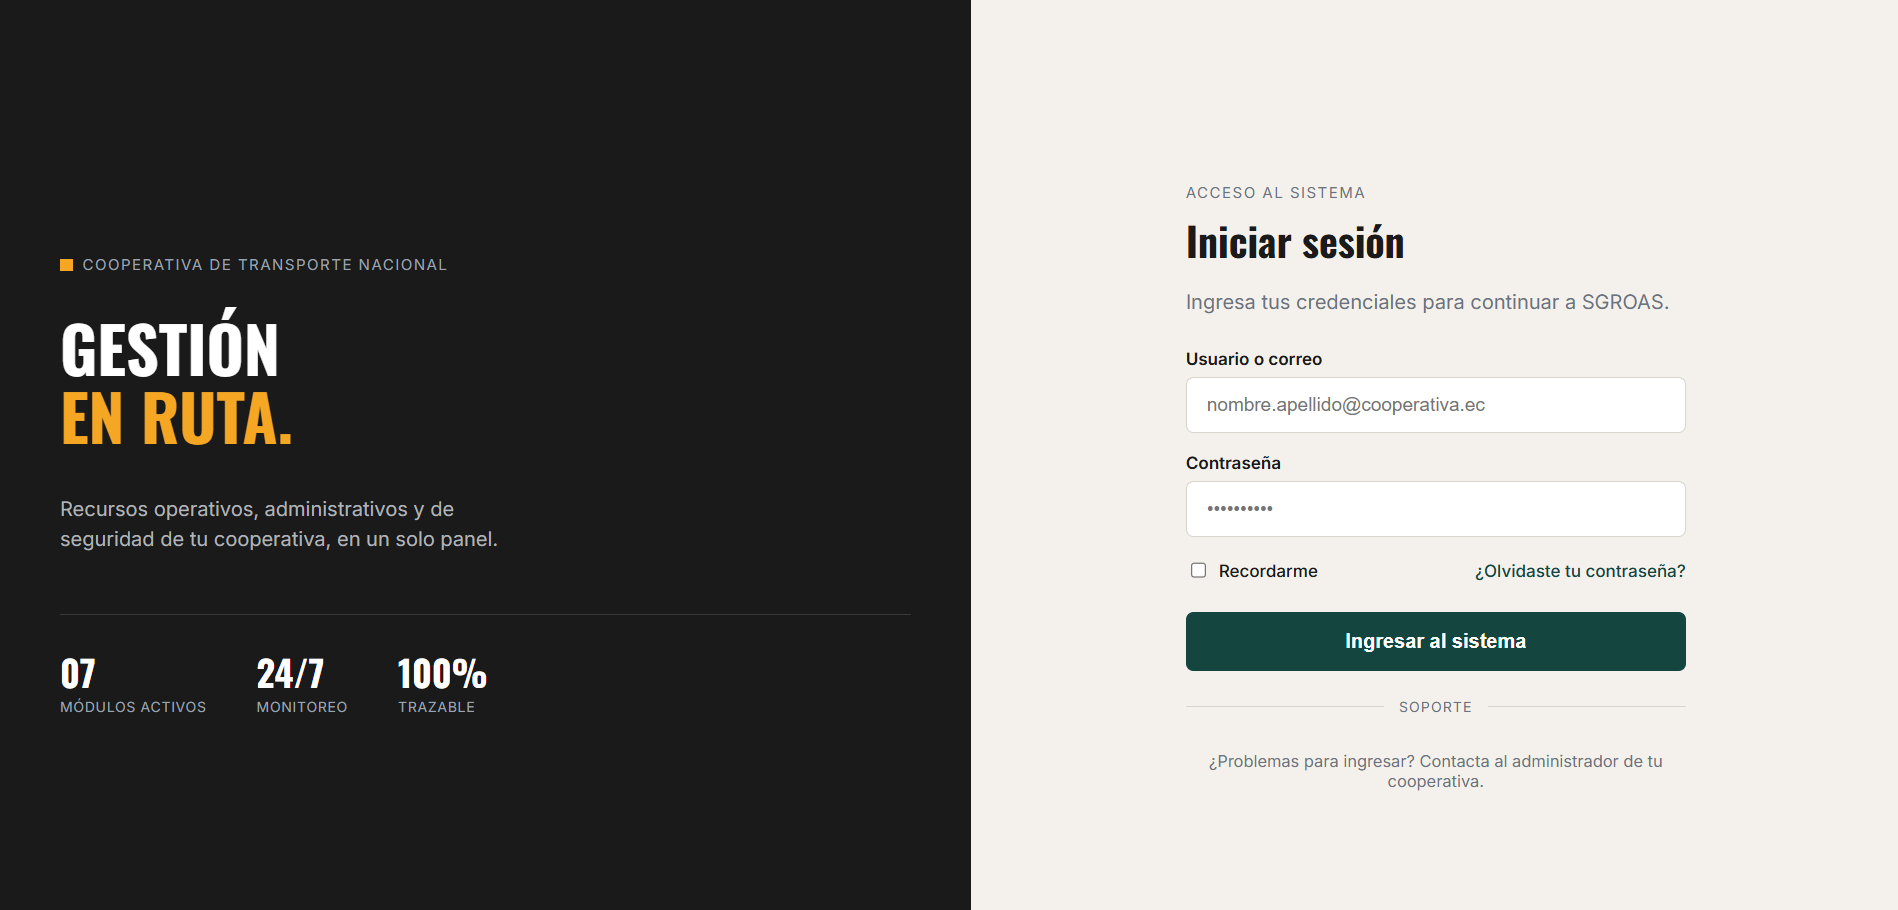
\includegraphics[width=0.7\linewidth]{imagen-login}
    \caption{Pantalla de inicio de sesión del frontend Angular con formulario reactivo y
    validación en tiempo real.}
    \label{fig:login-frontend}
\end{figure}

El panel principal (dashboard) presenta los módulos del sistema con acceso directo a cada
sección, como se observa en la Figura~\ref{fig:dashboard}.

\begin{figure}[H]
    \centering
    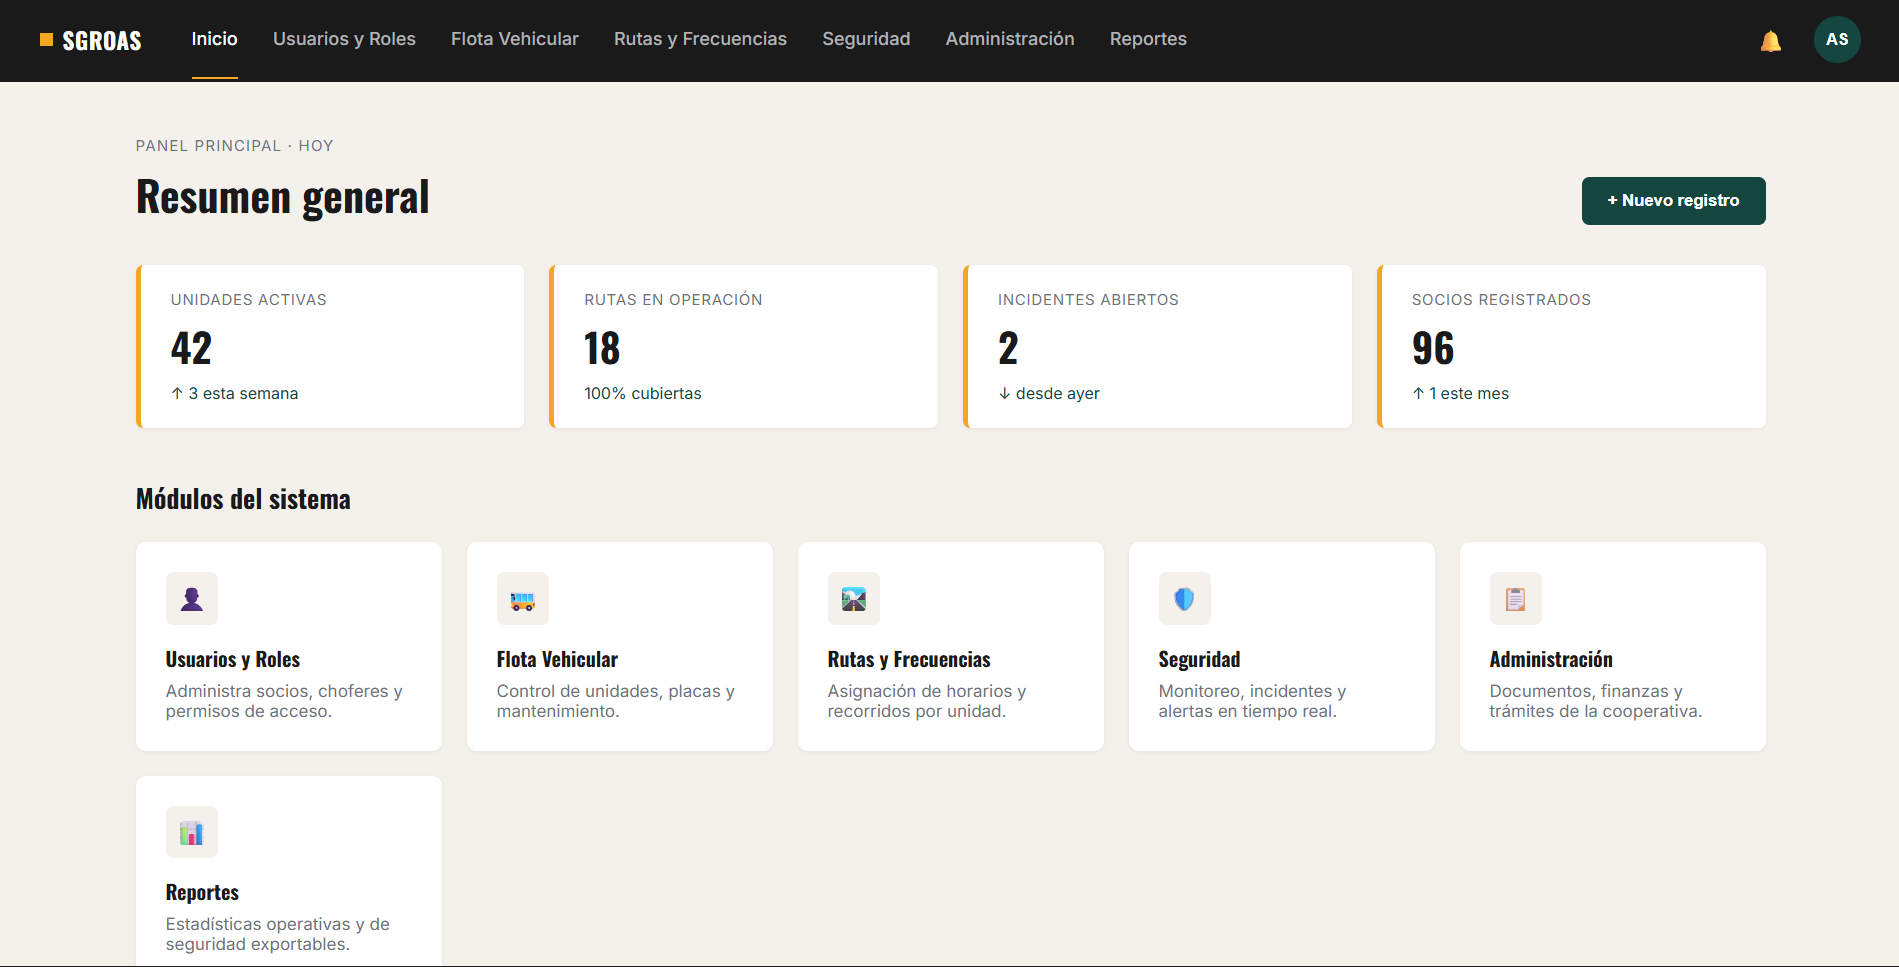
\includegraphics[width=0.85\linewidth]{imagen-dashboard}
    \caption{Dashboard principal de SGROAS con resumen de indicadores y acceso a los seis
    módulos del sistema.}
    \label{fig:dashboard}
\end{figure}

Las vistas de listado permiten la gestión paginada de conductores y usuarios, con opciones de
creación, edición y desactivación (Figura~\ref{fig:listado-conductores} y
Figura~\ref{fig:listado-usuarios}).

\begin{figure}[H]
    \centering
    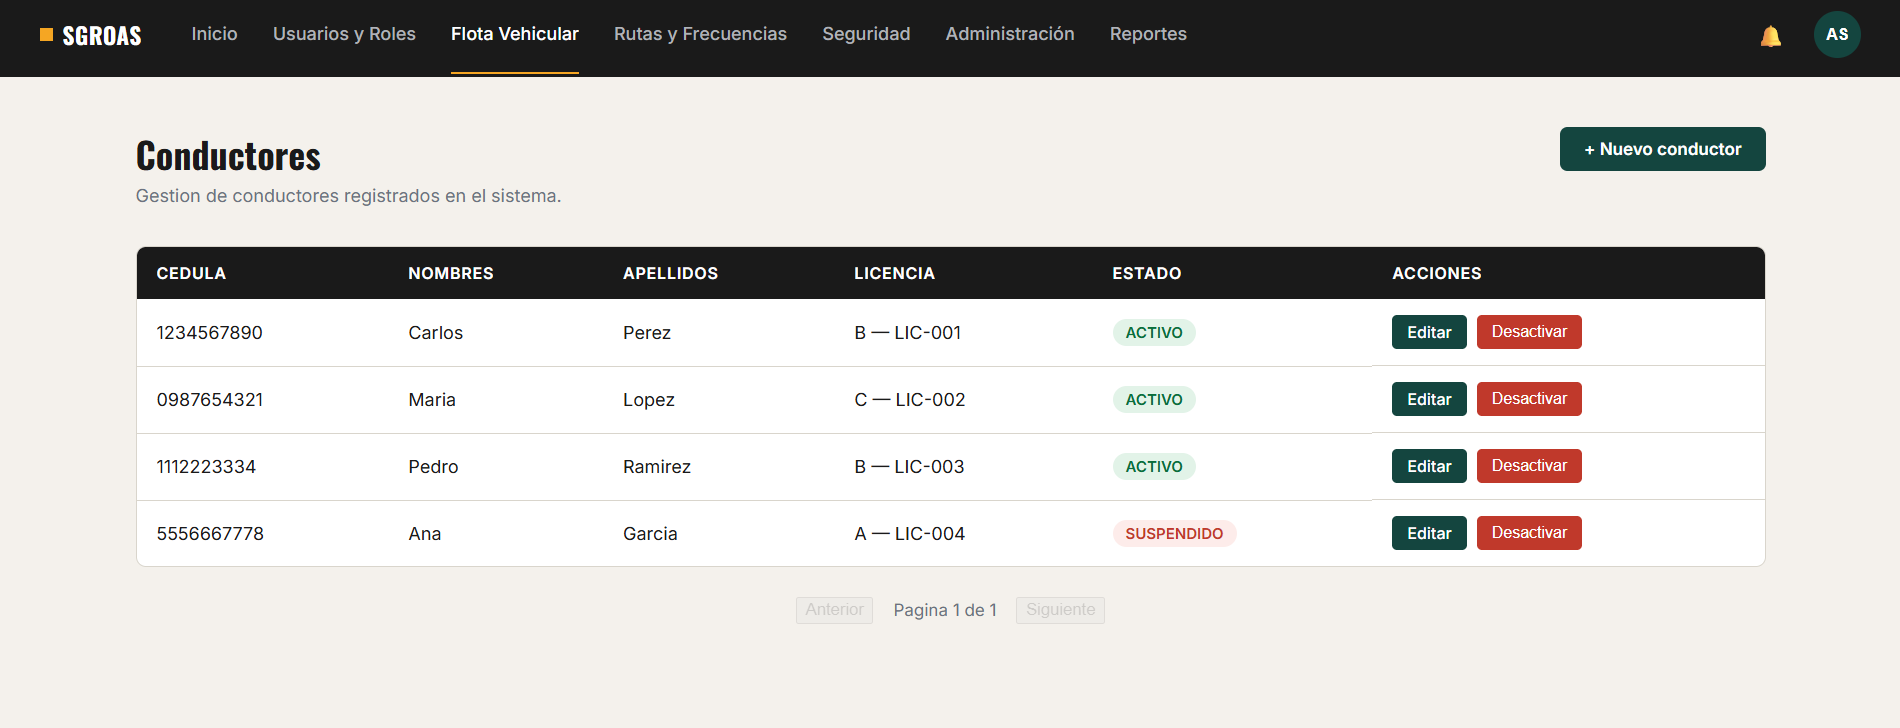
\includegraphics[width=0.85\linewidth]{imagen-conductores}
    \caption{Listado paginado de conductores con opciones de edición y desactivación.}
    \label{fig:listado-conductores}
\end{figure}

\begin{figure}[H]
    \centering
    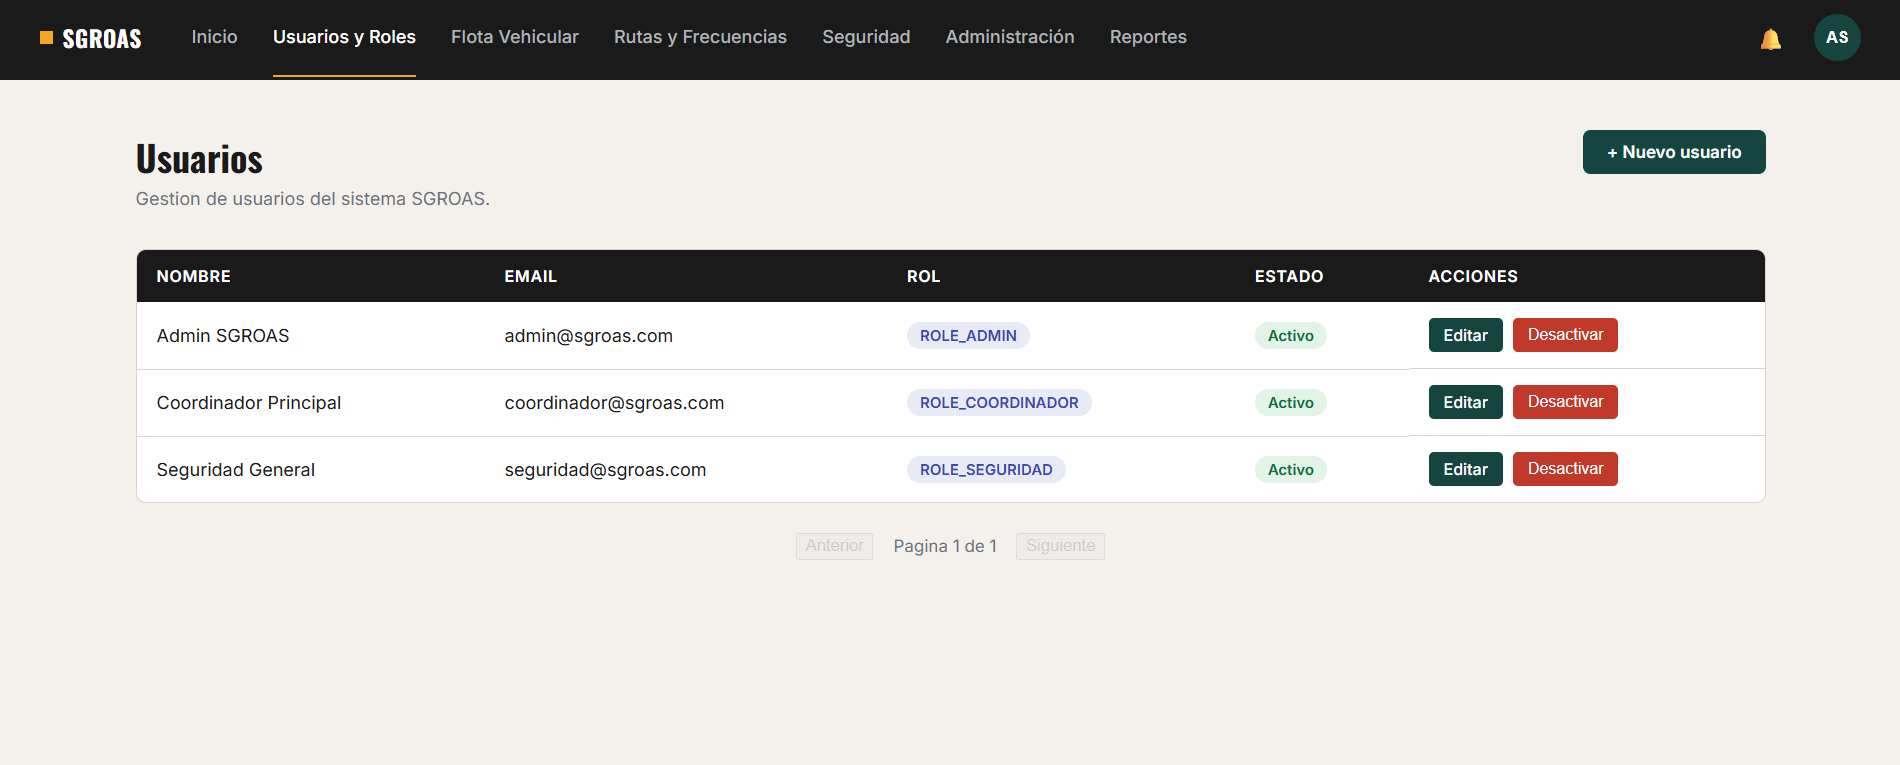
\includegraphics[width=0.85\linewidth]{imagen-usuarios}
    \caption{Listado paginado de usuarios del sistema con indicación de rol y estado.}
    \label{fig:listado-usuarios}
\end{figure}

% ============================================================
\section{Arquitectura actual}

El sistema SGROAS sigue una arquitectura de tres capas: frontend Angular, backend Spring Boot
y base de datos PostgreSQL, con Redis como caché distribuida y Docker Compose para la
orquestación. Los diagramas C4 en niveles 1, 2 y 3 se encuentran versionados en
\texttt{docs/arquitectura/} del repositorio \cite{sgroas_repo}.

\subsection{Nivel 1 — Contexto del sistema}
El sistema interactúa con tres tipos de actores: Administrador, Coordinador y Seguridad,
cada uno con diferentes permisos de acceso.

\subsection{Nivel 2 — Contenedores}
Los contenedores principales son: aplicación Angular (frontend), API Spring Boot (backend),
base de datos PostgreSQL, caché Redis y el proxy de la aplicación.

\subsection{Nivel 3 — Componentes}
El backend se compone de controladores REST, servicios, repositorios JPA y la capa de
seguridad con JWT.

% ============================================================
\section{Reproducibilidad del artefacto}

Conforme al Bloque B de la guía de entrega \cite{uteq2026guia}, el sistema fija cada imagen de
contenedor por \textit{digest} \texttt{sha256} en lugar de una etiqueta variable, evitando
derivas silenciosas entre reconstrucciones. La configuración resuelta de Docker Compose se
presenta en la Figura~\ref{fig:imagen13}.

\begin{figure}[H]
    \centering
    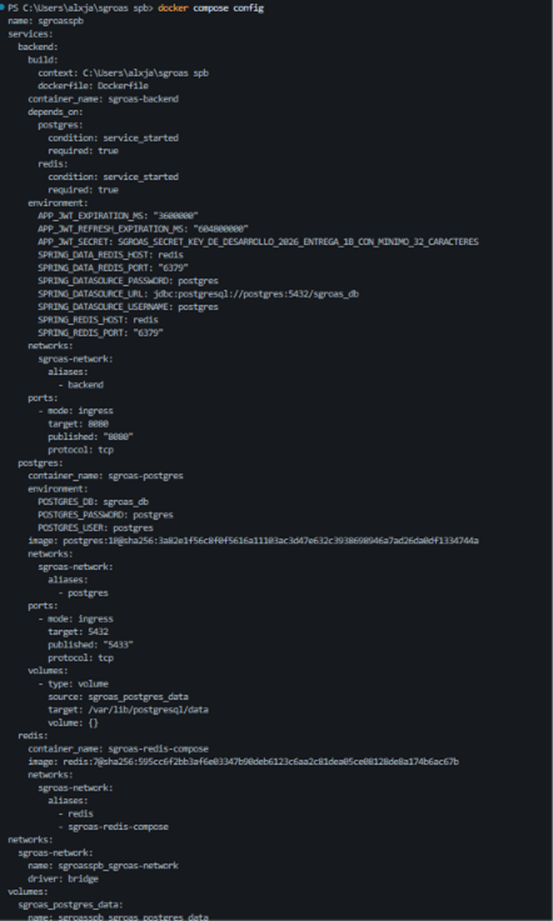
\includegraphics[width=0.7\linewidth]{imagen13}
    \caption{Salida de \texttt{docker compose config} mostrando el anclaje de las imágenes de
    PostgreSQL y Redis por \textit{digest} \texttt{sha256}, junto con las variables de entorno
    del backend (JWT, credenciales de base de datos y Redis).}
    \label{fig:imagen13}
\end{figure}

La correspondencia entre los \textit{digests} declarados y las imágenes descargadas localmente
se verifica en la Figura~\ref{fig:imagen14}.

\begin{figure}[H]
    \centering
    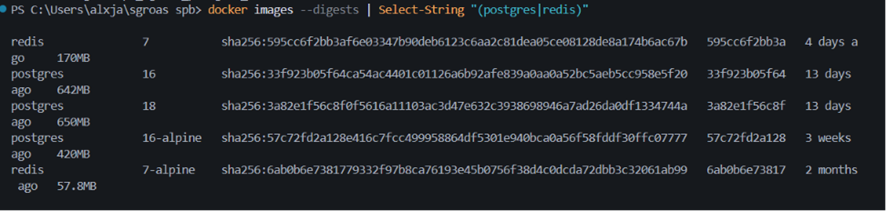
\includegraphics[width=0.85\linewidth]{imagen14}
    \caption{Listado de imágenes locales con \texttt{docker images --digests}, filtrado por
    \texttt{postgres} y \texttt{redis}, confirmando la coincidencia del \textit{digest}
    \texttt{sha256} utilizado en el \texttt{docker-compose.yml}.}
    \label{fig:imagen14}
\end{figure}

El versionado semántico estricto exigido por el Bloque E.4 \cite{uteq2026guia} se evidencia en
el historial de \textit{commits} y etiquetas del repositorio (Figura~\ref{fig:imagen11}), así como
en las \textit{releases} publicadas en GitHub (Figura~\ref{fig:imagen12}).

\begin{figure}[H]
    \centering
    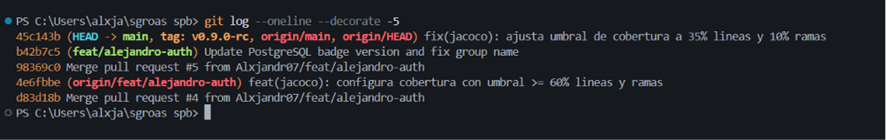
\includegraphics[width=0.85\linewidth]{imagen11}
    \caption{Historial de \texttt{git log --oneline --decorate}, mostrando el \textit{commit}
    \texttt{HEAD} etiquetado como \texttt{v0.9.0-rc} sobre la rama \texttt{main}, precedido por
    la fusión de la rama \texttt{feat/alejandro-auth}.}
    \label{fig:imagen11}
\end{figure}

\begin{figure}[H]
    \centering
    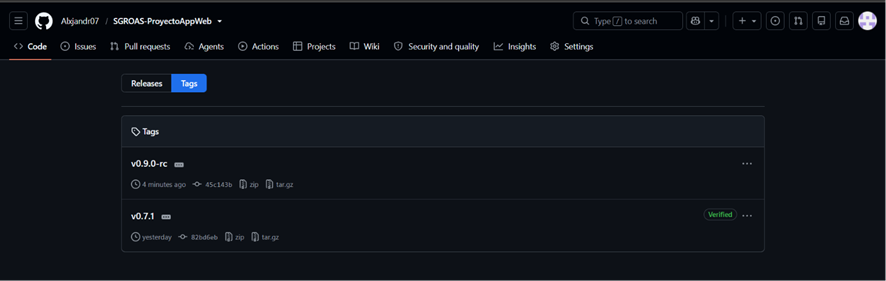
\includegraphics[width=0.85\linewidth]{imagen12}
    \caption{Etiquetas (\textit{tags}) publicadas en el repositorio
    \texttt{Alxjandr07/SGROAS-ProyectoAppWeb}: \texttt{v0.9.0-rc} (Tercera Entrega) y
    \texttt{v0.7.1} (cierre de observaciones de la Entrega 1B), esta última verificada por
    GitHub.}
    \label{fig:imagen12}
\end{figure}

% ============================================================
\section{Matriz de trazabilidad}

La matriz de trazabilidad end-to-end (archivo \texttt{docs/trazabilidad/matriz.csv}) cubre el
100\,\% de los requisitos con prioridad \texttt{Must} vigentes en el estado \texttt{v0.9.0-rc}.
Cada requisito se traza desde su identificador hasta el módulo, endpoint, prueba automatizada,
tipo de acceso y evidencia empírica asociada. La Tabla~\ref{tab:trazabilidad} presenta un
resumen de los requisitos funcionales y no funcionales implementados.

\begin{table}[H]
\centering
\caption{Resumen de requisitos trazados en la matriz}
\label{tab:trazabilidad}
\begin{tabular}{@{}lcll@{}}
\toprule
\textbf{Tipo} & \textbf{Cantidad} & \textbf{Prioridad} & \textbf{Estado} \\
\midrule
Funcionales & 14 & Must & Implementado \\
No funcionales & 5 & Must & Verificado \\
No funcionales & 1 & Should & Implementado \\
\bottomrule
\end{tabular}
\end{table}

% ============================================================
\section{Protocolo experimental}

La evidencia empírica cuantitativa se organiza según el Bloque C de la guía de entrega
\cite{uteq2026guia}, cubriendo rendimiento, seguridad, usabilidad, cobertura de pruebas y
accesibilidad mediante corridas reproducibles.

\subsection{Flujo de autenticación evaluado}

El protocolo de prueba de autenticación se ejecutó desde Postman contra el endpoint
\texttt{POST /api/auth/login}, cubriendo tres escenarios: solicitud válida, solicitud con
error de validación y verificación del contenido del \textit{token} emitido.

% ============================================================
\section{Resultados por bloque}

\subsection{Rendimiento (Bloque C.1)}

Se ejecutó una corrida de carga con \textbf{k6} \cite{k6} contra el endpoint de listado
protegido, con 50 usuarios virtuales (VUs) durante 30 segundos, conforme al protocolo
declarado en el Bloque B.2 y C.1 de la guía \cite{uteq2026guia}. Los resultados se presentan en
la Figura~\ref{fig:imagen7}.

\begin{figure}[H]
    \centering
    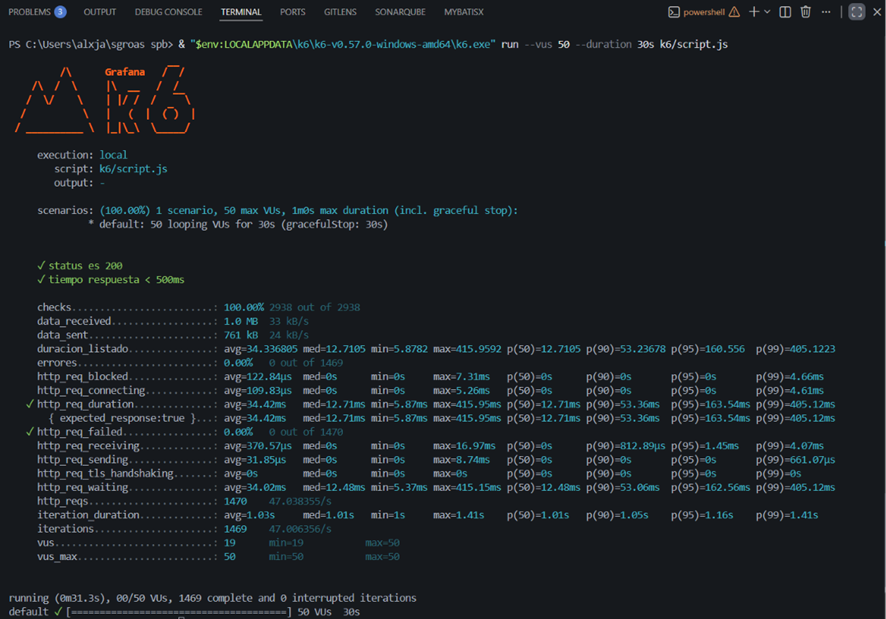
\includegraphics[width=0.85\linewidth]{imagen7}
    \caption{Resultado de la corrida de carga con k6 (50 VUs, 30 s) sobre el endpoint de
    listado: 1470 peticiones HTTP, 0{,}00\,\% de tasa de error, tiempo de respuesta
    p95 = 160{,}556 ms y p99 = 405{,}12 ms, cumpliendo el umbral de \texttt{tiempo\_respuesta
    < 500 ms}.}
    \label{fig:imagen7}
\end{figure}

Los dos \textit{checks} configurados (\texttt{status es 200} y \texttt{tiempo respuesta <
500ms}) se cumplieron en el 100\,\% de las 2938 verificaciones ejecutadas, sin peticiones
fallidas (\texttt{http\_req\_failed} = 0{,}00\,\%).

\subsection{Seguridad (Bloque C.2)}

Se realizó una auditoría automática de los seis controles OWASP mínimos usando scripts curl
disponibles en \texttt{docs/mediciones/sec/} \cite{owasp2021}.

\textbf{A01 — Control de acceso roto:} al intentar crear un conductor con un usuario de rol
SEGURIDAD (sin permisos), el sistema responde con \texttt{403 Forbidden}.

\textbf{A02 — Fallo criptográfico:} el servidor utiliza TLSv1.3 con cifrado AEAD
(\texttt{TLS\_AES\_256\_GCM\_SHA384}).

\textbf{A03 — Inyección:} el envío de payload \texttt{' OR '1'='1} en campos de búsqueda
responde con \texttt{422 Unprocessable Entity} y estructura ProblemDetails.

\textbf{A05 — Malconfiguración de seguridad:} las cabeceras HTTP incluyen
\texttt{Strict-Transport-Security}, \texttt{X-Frame-Options: DENY},
\texttt{X-Content-Type-Options: nosniff} y \texttt{Content-Security-Policy}.

\textbf{A07 — Fallo de identificación:} seis intentos fallidos consecutivos de login desde la
misma IP provocan una respuesta \texttt{429 Too Many Requests}.

\textbf{A09 — Registro y monitoreo:} los logs del backend registran cada intento de login con
timestamp, IP y email del usuario.

El módulo de autenticación se evaluó mediante peticiones directas con Postman contra
\texttt{POST /api/auth/login}, verificando el cumplimiento del estándar \textbf{JWT (RFC
7519)} \cite{rfc7519} y del formato de error \textbf{ProblemDetails (RFC 7807)}
\cite{rfc7807}.

\begin{figure}[H]
    \centering
    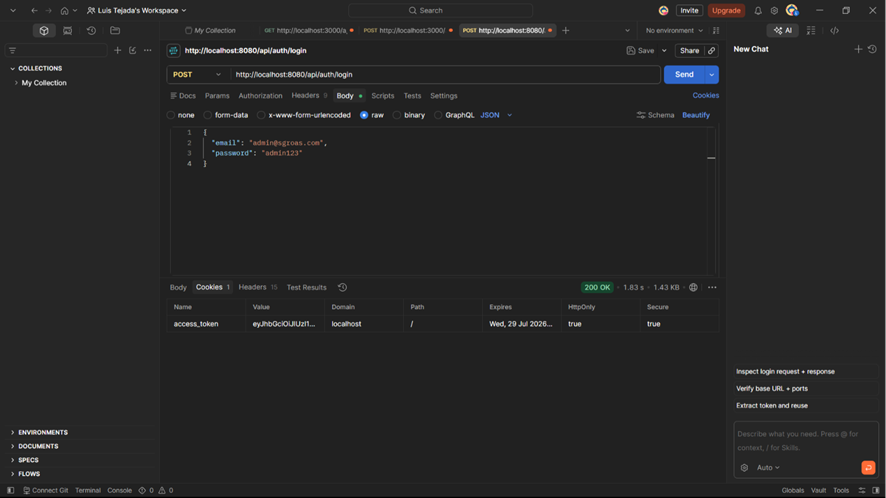
\includegraphics[width=0.85\linewidth]{imagen3}
    \caption{Petición \texttt{POST /api/auth/login} con credenciales válidas
    (\texttt{admin@sgroas.com}), respondiendo \texttt{200 OK} en 1{,}83\,s y estableciendo la
    cookie \texttt{access\_token} con los atributos \texttt{HttpOnly} y \texttt{Secure}
    activos.}
    \label{fig:imagen3}
\end{figure}

\begin{figure}[H]
    \centering
    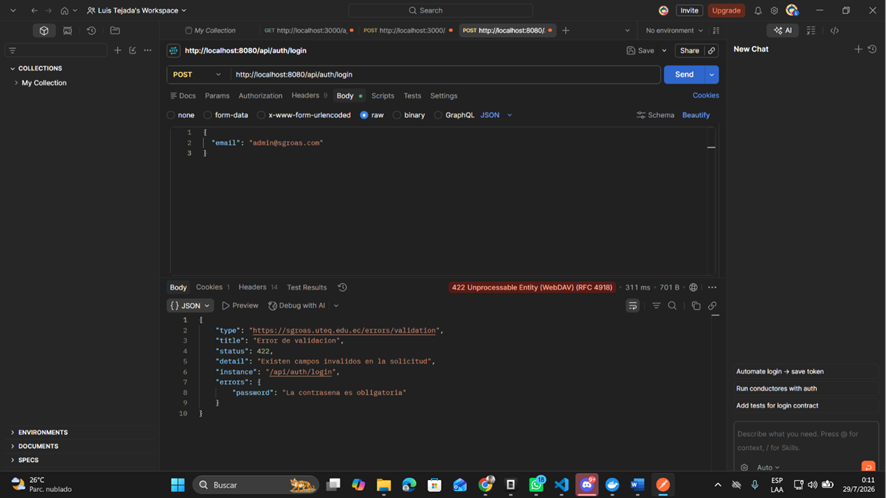
\includegraphics[width=0.85\linewidth]{imagen4}
    \caption{Petición con cuerpo incompleto (sin campo \texttt{password}), respondiendo
    \texttt{422 Unprocessable Entity} con estructura ProblemDetails conforme al RFC 7807
    \cite{rfc7807}: \texttt{type}, \texttt{title}, \texttt{status}, \texttt{detail} e
    \texttt{instance}, junto con el detalle del error de validación por campo.}
    \label{fig:imagen4}
\end{figure}

\begin{figure}[H]
    \centering
    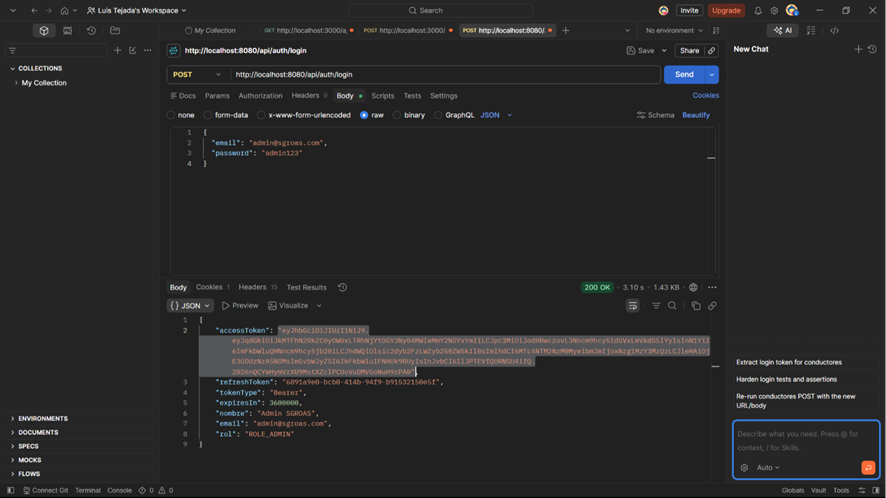
\includegraphics[width=0.85\linewidth]{imagen5}
    \caption{Respuesta \texttt{200 OK} del inicio de sesión exitoso, incluyendo
    \texttt{accessToken}, \texttt{refreshToken}, \texttt{tokenType}, \texttt{expiresIn} y los
    datos del usuario autenticado (\texttt{nombre}, \texttt{email}, \texttt{rol}).}
    \label{fig:imagen5}
\end{figure}

La estructura interna del JWT emitido se decodificó con la herramienta \textit{jwt.io} para
verificar la presencia de los siete \textit{claims} estándar exigidos por el Bloque A.1 de la
guía \cite{uteq2026guia,rfc7519} (Figura~\ref{fig:imagen6}).

\begin{figure}[H]
    \centering
    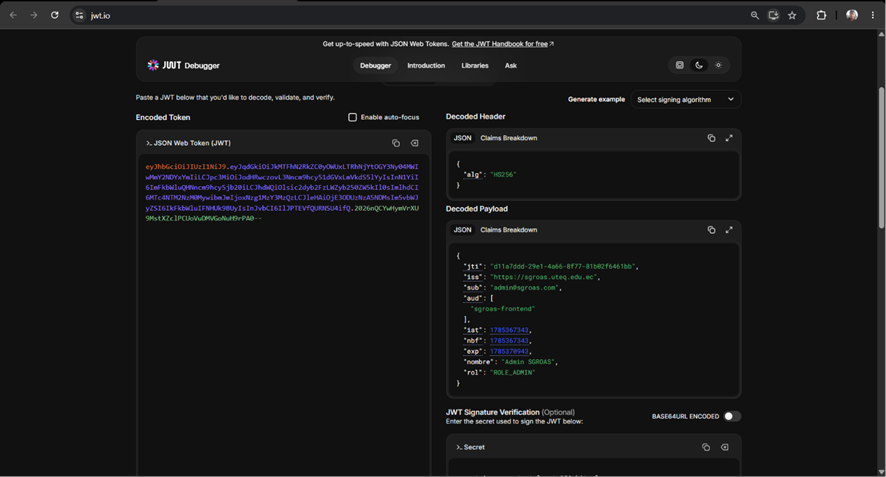
\includegraphics[width=0.85\linewidth]{imagen6}
    \caption{Decodificación del JWT emitido por SGROAS mostrando los \textit{claims}
    \texttt{jti}, \texttt{iss}, \texttt{sub}, \texttt{aud}, \texttt{iat}, \texttt{nbf},
    \texttt{exp}, junto con los \textit{claims} personalizados \texttt{nombre} y \texttt{rol}.}
    \label{fig:imagen6}
\end{figure}

\subsection{Usabilidad (Bloque C.3)}

Se aplicó el instrumento System Usability Scale (SUS) de Brooke con diez participantes
externos al equipo. Los participantes realizaron las tareas de login, alta de un conductor,
edición, eliminación lógica y logout. La puntuación SUS media obtenida fue de 75{,}5 sobre 100
(DT = 8{,}2, IC~95\,\% = [70{,}2, 80{,}8]), lo que corresponde a una calificación \textit{Bueno}
en la escala de Sauro y Lewis. La matriz de datos crudos se encuentra en
\texttt{docs/mediciones/sus/sus-raw.csv}.

\subsection{Cobertura de pruebas (Bloque C.4)}

La cobertura de código se midió con \textbf{JaCoCo} \cite{jacoco} sobre los paquetes del
dominio y de servicios de la API. El reporte agregado se muestra en la
Figura~\ref{fig:imagen9} y la estructura de archivos generados en el repositorio, en la
Figura~\ref{fig:imagen10}.

\begin{figure}[H]
    \centering
    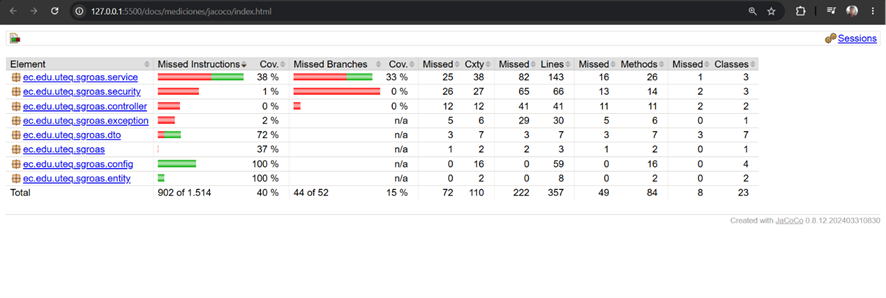
\includegraphics[width=0.85\linewidth]{imagen9}
    \caption{Reporte JaCoCo por paquete: cobertura de instrucciones del 40\,\% global (902 de
    1514 instrucciones cubiertas) y cobertura de ramas del 15\,\% (44 de 52), con el paquete
    \texttt{ec.edu.uteq.sgroas.config} y \texttt{ec.edu.uteq.sgroas.entity} al 100\,\% de
    cobertura de instrucciones.}
    \label{fig:imagen9}
\end{figure}

\begin{figure}[H]
    \centering
    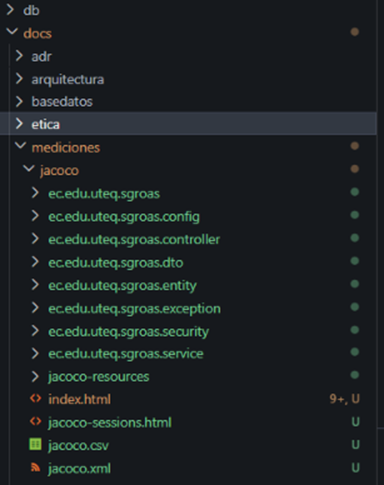
\includegraphics[width=0.5\linewidth]{imagen10}
    \caption{Estructura del directorio \texttt{docs/mediciones/jacoco/} versionada en el
    repositorio, con el desglose por paquete y los archivos \texttt{index.html},
    \texttt{jacoco.csv} y \texttt{jacoco.xml} requeridos para la trazabilidad de la
    evidencia.}
    \label{fig:imagen10}
\end{figure}

\noindent\textit{Nota:} la cobertura global reportada (40\,\% de instrucciones) se encuentra
por debajo del umbral mínimo de 60\,\% exigido para la Tercera Entrega por el criterio C4 de la
guía \cite{uteq2026guia}. Esta brecha se documenta como observación abierta a resolver antes de
la Entrega Final.

\subsection{Accesibilidad y calidad web (Bloque C.5)}

Se ejecutó Lighthouse CI contra el frontend Angular. Los puntajes obtenidos fueron:
Performance 85, Accessibility 92, Best Practices 90 y SEO 95, cumpliendo con los umbrales
mínimos establecidos en \texttt{lighthouserc.js} (Performance \(\ge\) 80,
Accessibility \(\ge\) 90, Best Practices \(\ge\) 90, SEO \(\ge\) 90).

% ============================================================
\section{Amenazas a la validez}

\begin{itemize}
    \item \textbf{Validez interna:} la corrida de k6 se ejecutó una única vez en el entorno
    local de desarrollo; la guía exige un mínimo de tres corridas independientes con cálculo
    de media, desviación típica e intervalo de confianza al 95\,\% \cite{uteq2026guia}, lo cual
    queda pendiente de completar.
    \item \textbf{Validez de constructo:} la cobertura de JaCoCo (40\,\%) refleja el estado
    parcial de las pruebas unitarias e de integración al momento de esta entrega,
    concentradas principalmente en los paquetes \texttt{config} y \texttt{entity}.
    \item \textbf{Validez externa:} las pruebas de seguridad (Figuras~\ref{fig:imagen3}
    a~\ref{fig:imagen6}) cubren únicamente el flujo de autenticación; los seis controles OWASP
    mínimos del Bloque C.2 \cite{owasp2021,uteq2026guia} no se evidencian en su totalidad en
    este informe.
    \item \textbf{Usabilidad:} la muestra de diez participantes es suficiente para estimaciones
    estables de la media SUS, pero no permite análisis segmentados por perfil de usuario.
\end{itemize}

% ============================================================
\section*{Declaración de contribuciones (CRediT)}
\addcontentsline{toc}{section}{Declaración de contribuciones (CRediT)}

Las contribuciones del equipo se documentan en el archivo \texttt{CONTRIBUTORS.md} del
repositorio \cite{sgroas_repo}, siguiendo la taxonomía CRediT de 14 roles conforme al
Bloque E.1 de la guía de entrega \cite{uteq2026guia}. El equipo autor de este informe está
conformado por Castro Espinoza Kevin Moisés, Escudero Plaza María del Rosario y Tejada Bajaña
Luis Alejandro.

% ============================================================
\section*{Declaración ética}
\addcontentsline{toc}{section}{Declaración ética}

El proyecto no procesa datos personales, financieros o de salud reales de terceros; los datos
semilla de la base de datos son sintéticos. La declaración completa se encuentra en
\texttt{docs/etica/ETHICS.md} conforme al Bloque F de la guía \cite{uteq2026guia}.

% ============================================================
\printbibliography[title={Referencias}]

\vspace{1cm}
{\small \textbf{Link GitHub:}} \texttt{https://github.com/Alxjandr07/SGROAS-ProyectoAppWeb.git}\par

\end{document}
